\documentclass[runningheads]{llncs}

\usepackage[T1]{fontenc}
\usepackage{graphicx}

% to display URLs in blue roman font according to Springer's eBook style:
%\usepackage{color}
%\renewcommand\UrlFont{\color{blue}\rmfamily}
%\urlstyle{rm}

\begin{document}
\title{Computer Networks Project \\ Romanian railways}

\author{P. Braha\inst{1}\orcidID{0009-0001-3636-2455}}
\authorrunning{F. Author et al.}
\institute{Alexandru Ioan Cuza University, Iasi IS 700221, Romania
\email{petrubraha@gmail.com}\\
\url{https://github.com/petru-braha}}

\maketitle

\begin{abstract} This work contains an overview of the client-server paradigm offering, to the public transport companies, a concrete (and open source) informational system connected with potential clients. This system provides a service that notifies the consumers about the traveling schedule, the available means of transport (e. g. trains) to their time and location alongside with additional information such as status of departure/arrival and vehicle identification. Any user has the possibility to report late arrivals in a controlled manner such that the misleading (and wrong) data provided by them, is checked. The application runs concurrently and achieves great speed in communication with its clients, without impacting the correctness of the responses. The security of the system is accomplished by having two different running servers at different locations. If any of them fails, there exists a guaranteed back-up. The communication between them is not omitted. This paper is relevant in the actual industry showcasing my skills for system management. (150 - 250).

\keywords{TCP \and UDP \and I/O multiplexing \and Concurrency.}
\end{abstract}

%%------------------------------------------------
%%------------------------------------------------

\section{Introduction}

The current document dives directly into the technologies used. The next section introduces details about concurrency, transport protocols, and descriptor manipulation. Chapter 3 covers the structure of the server application, and some visualizations are briefly explained to create a solid understanding of the communication protocol. Following this, all details, experiments, and observation about this implementation are explored, as well as the application API. The conclusions will summarize my project and propose some real scenarios where the RR application could be used.

\subsection{Motivation}

The repository is a matter of personal pasion for the "Computer Networks" course. Officially, it is known as laboratory homework, but its goal is far higher than this. My motivation was to create a application that could have real life usage. My wish is to consider this project a potential example for future implementations. Being encouraged to provide creative ideas everything here was born.

\section{Applied Technologies}

\subsection{Concurrency strategies}

A number of strategies were evaluated and tested before the final choice:
\begin{itemize}
    \item preforked execution 
    \item prethreaded execution 
    \item child process per client
    \item thread per client
    \item i/o multiplexing with blocking calls
    \item i/o multiplexing with non-blocking calls
\end{itemize}

- thread over child process
	- smaller cost (course example of 50.000)
	- there can be a lot of writes on the server data
	- the child process will copy by ref but threads plays with the parent process' variables themselves

what about prethreaded VS thread per client?

\subsection{Transport protocol}

The communication uses a combination of TCP and UDP for the transport protocol. Their advantages were exploited for the adequate situation.
The TCP protocol is used for the commands that are responsible for influencing the server's data. It is a secure protocol TCP providing acknoledgements for all the transmited messages. On the other hand, it implies an increased amount of time which is the reason of UDP usage. For important messages we're taking no risk in the alteration of the data, but for small interogations it is prefered a faster communication. If the communication fails, it can be simply restarted by the consumer. 

If the data sent by the client is altered => wrong number of minutes => the schedule becomes incorrect. it's okay if the client's query is not received from the first attempt, but the data received by him has to be not affected and accurate.

a. client uses tcp to server when sending data
b. client uses udp to server when sending queries
c. server uses tcp to client when sending data

\subsection{I/O Multiplexing}

- using select() and unblocking I/O operations is the fastest strategy. how can i make it faster? (fastest <- course)

There will be a global I/O multiplexing, each thread accessing it.

a. the sever uses i/o multiplexing and serves the ready file descriptors concurently using threads

\section{Application Structure}

diagram
Expose the concepts used in modeling and present a detailed diagram of the application.

\begin{table}
    \caption{Table captions should be placed above the
    tables.}\label{tab1}
    \begin{tabular}{|l|l|l|}
    \hline
    Heading level &  Example & Font size and style\\
    \hline
    Title (centered) &  {\Large\bfseries Lecture Notes} & 14 point, bold\\
    1st-level heading &  {\large\bfseries 1 Introduction} & 12 point, bold\\
    2nd-level heading & {\bfseries 2.1 Printing Area} & 10 point, bold\\
    3rd-level heading & {\bfseries Run-in Heading in Bold.} Text follows & 10 point, bold\\
    4th-level heading & {\itshape Lowest Level Heading.} Text follows & 10 point, italic\\
    \hline
    \end{tabular}
    \end{table}
    
    
    \noindent Displayed equations are centered and set on a separate
    line.
    \begin{equation}
    x + y = z
    \end{equation}
    Please try to avoid rasterized images for line-art diagrams and
    schemas. Whenever possible, use vector graphics instead (see
    Fig.~\ref{fig1}).
    
    \begin{figure}
    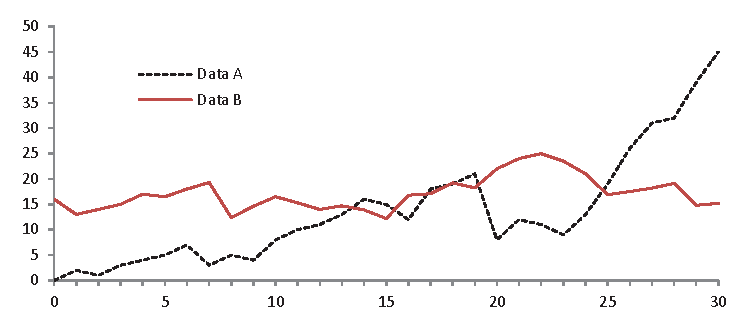
\includegraphics[width=\textwidth]{fig1.eps}
    \caption{A figure caption is always placed below the illustration.
    Please note that short captions are centered, while long ones are
    justified by the macro package automatically.} \label{fig1}
    \end{figure}
    
    \begin{theorem}
    This is a sample theorem. The run-in heading is set in bold, while
    the following text appears in italics. Definitions, lemmas,
    propositions, and corollaries are styled the same way.
    \end{theorem}
    

\section{Implementation Aspects}

time experiments
extra server for security
innovative sections of the project code 
describe the api - describe real usage scenarios.

\subsection{Definitions and Decisions}

The time of the application is the current Romania time.
- an itinerary is from point A to point B and no other points exists between these two. If that would be the case then extra complexity would be added to the logic of the application.

- locations types
    - departures
    - arrivals

- times types
    - confirmed departure time
    - estimated departure time
    - confirmed arrival time
    - estimated arrival time


\subsection{Application protocol}

The data is composed of:
\begin{itemize}
    \item routes
    \item departure/arrival status
    \item delays
    \item arrival estimation
\end{itemize}

The server is responsable for:
\begin{itemize}
    \item sends data to clients
    \item receives data from xml files
    \item receives delays from clients
    \item updates dalays, arrival estimation

\end{itemize}
    
The client application contains 5 commands

\begin{itemize}
    \item [id train, time departure estimated, time arrival estimated, status] routes(location departure, location arrival)
\end{itemize}


- function model: return_type name_function parameter(s)
- estimated times = initial times defined by the generated schedule
- confirmed times = estimated times +/- delays (depends if the train arrives earlier or later)
- status has two fields - each indicates whether it has left or arrived
- a clear distinction is made between the word estimated and confirmed. The former has an information initializing character, and while the server is running for that day estimated emphasizes that the information


\section{Conclusions}

tcp and udp protocol


\subsection{speed}

tcp/udp
i/o multiplexing
concurrency

\subsection{corectness}

tcp protocol

\subsection{security}

\begin{credits}
    \subsubsection{\ackname} A bold run-in heading in small font size at the end of the paper is
    used for general acknowledgments, for example: This study was funded
    by X (grant number Y).
    e
    \subsubsection{\discintname}
    It is now necessary to declare any competing interests or to specifically
    state that the authors have no competing interests. Please place the
    statement with a bold run-in heading in small font size beneath the
    (optional) acknowledgments\footnote{If EquinOCS, our proceedings submission
    system, is used, then the disclaimer can be provided directly in the system.},
    for example: The authors have no competing interests to declare that are
    relevant to the content of this article. Or: Author A has received research
    grants from Company W. Author B has received a speaker honorarium from
    Company X and owns stock in Company Y. Author C is a member of committee Z.
    \end{credits}
    

%%------------------------------------------------
%%------------------------------------------------
%citations: square brackets and consecutive numbers. Citations using labels or the author/year
%convention are also acceptable. The following bibliography provides
%a sample reference list with entries for journal
%aarticles~\cite{ref_article1}, an LNCS chapter~\cite{ref_lncs1}, a
%abook~\cite{ref_book1}, proceedings without editors~\cite{ref_proc1},
%aand a homepage~\cite{ref_url1}. \cite{ref_article1,ref_book1,ref_proc1,ref_url1}.

% \bibliographystyle{splncs04}
% \bibliography{mybibliography}

\begin{thebibliography}{8}
\bibitem{ref_article1}
Author, F.: Article title. Journal \textbf{2}(5), 99--110 (2016)

\bibitem{ref_lncs1}
Author, F., Author, S.: Title of a proceedings paper. In: Editor,
F., Editor, S. (eds.) CONFERENCE 2016, LNCS, vol. 9999, pp. 1--13.
Springer, Heidelberg (2016). \doi{10.10007/1234567890}

\bibitem{ref_book1}
Author, F., Author, S., Author, T.: Book title. 2nd edn. Publisher,
Location (1999)

\bibitem{ref_proc1}
Author, A.-B.: Contribution title. In: 9th International Proceedings
on Proceedings, pp. 1--2. Publisher, Location (2010)

\bibitem{ref_url1}
LNCS Homepage, \url{http://www.springer.com/lncs}, last accessed 2023/10/25
\end{thebibliography}
\end{document}
